\section{Mekong}

Date: 26/06/2008

\begin{multicols}{2}

Mékong, Mékong... ça me dit quelque chose...

Mais oui c'est bien ça, le fleuve qui part de Chine, fait la frontière entre le la Thaïlande et le Laos puis va au Cambodge. Je suis parti de Pai en bus direction Chiang Khong, ville Thai faisant face a Huay Xay, ville Laotienne. C'est donc là que j'ai passé les deux postes d'émigration et d'immigration, puis je me suis enbarqué sur un bateau pour descendre sur le Mékong vers Luang Prabang, en deux jours.

Pour cet article, exceptionnelement je ne vous propose que des photos, en effet le recit de ces deux jours tient en deux mot : chill out

\hspace*{-0.65cm}
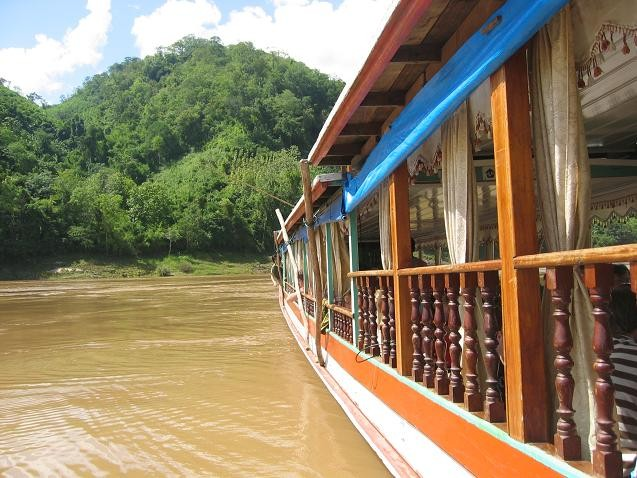
\includegraphics[width=4.8cm]{articles/Mekong/1214473370zy1a.jpg}
Le bateau vu en longueur

\hspace*{-0.65cm}
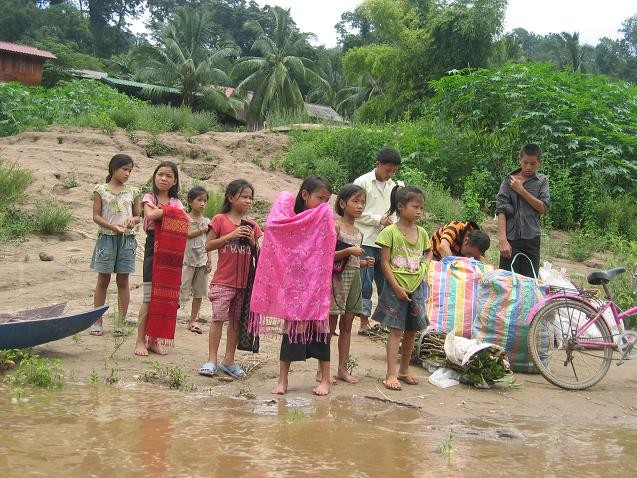
\includegraphics[width=4.8cm]{articles/Mekong/12144733896AMi.jpg}
Des enfants sur la berge

\hspace*{-0.65cm}
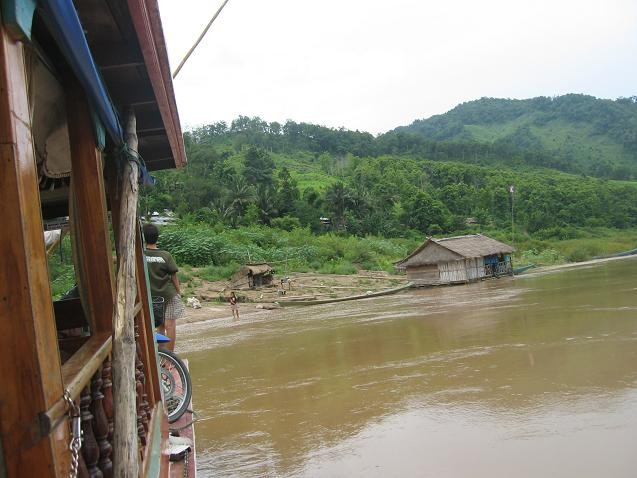
\includegraphics[width=4.8cm]{articles/Mekong/1214473395mtro.jpg}
Encore une escale

\hspace*{-0.65cm}
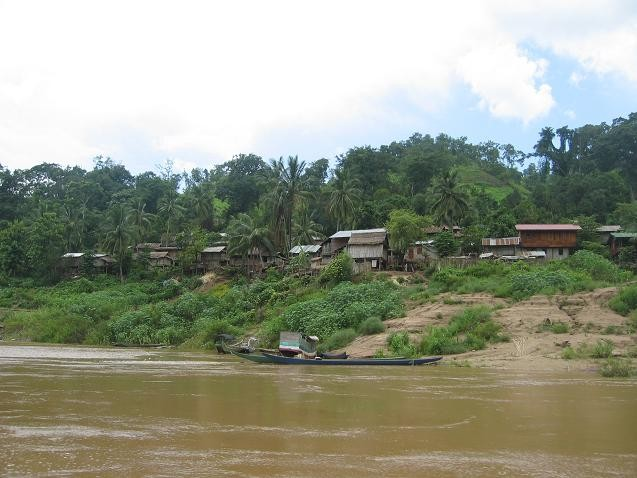
\includegraphics[width=4.8cm]{articles/Mekong/1214473400ezNu.jpg}
Un village sur la côte

\hspace*{-0.65cm}
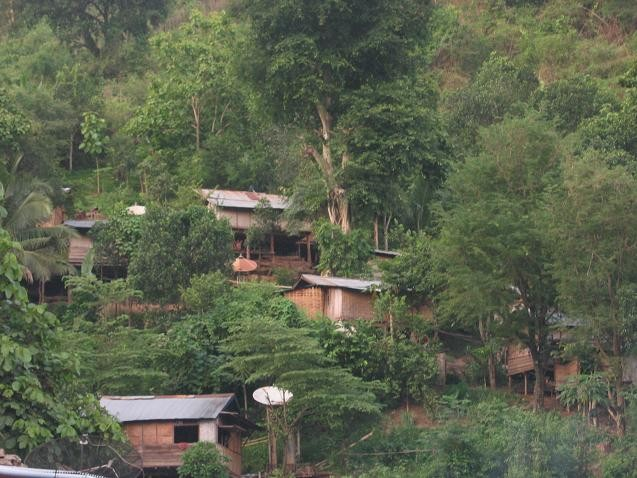
\includegraphics[width=4.8cm]{articles/Mekong/1214473407uNUm.jpg}
Escale du soir

\end{multicols}
